\subsection{Intercept}

\subsubsection*{Simple Definitions}

\begin{itemize}
  \item Offset: driving to the left or right of a target instead of right at it

  \item VID: Visual Identification

  \item Stern conversion: An intercept that arrives at displaced side of the
    bogey leaving 40000 feet to turn to his tail

  \item Geometry: Loose term describing the paths to be taken by multiple
    aircraft in relation to each other

  \item Stiffarm: hard turn to place the bandit 50 degrees on the cold side of
    the radar (point at his exhausts)

\end{itemize}

\subsubsection*{Scenario 1: Direct engagement, HOSTILE classification}

FL RIO will set geometry for the intercept so as to arrive in 40nm at co
altitude, nose hot at engagement speed of 400kts in the shortest distance. VID
and merge is not desired as target will be shot outside Visual Range.

An offset WILL be taken of at least 20 degrees left or right of the bandit,
seeking to obtain favourable positional advantage

\subsubsection*{Scenario 2: VID intercept, Stern conversion, Bogey
  classification not upgraded}

\sidebyside{0.6}{%
  FL RIO will set geometry to arrive within VID of the bandit at co alt with
  40000 feet turning room of offset to perform a single turn onto the bandits
  tail

  \subsubsection*{Stiffarming}

  \begin{itemize}
    \item Reduce closure speed
    \item Seek favourable position
    \item Determine Bogeys intentions
  \end{itemize}

  \boxed{
    Note: Offsets are discussed in detail in the A-A TTP 1. For now, pick the
    cold side of the bandit or favourable geometry towards chicks, friendly
    SAMs, or more often away from FLOT, hostile SAMs
  }
}{%
  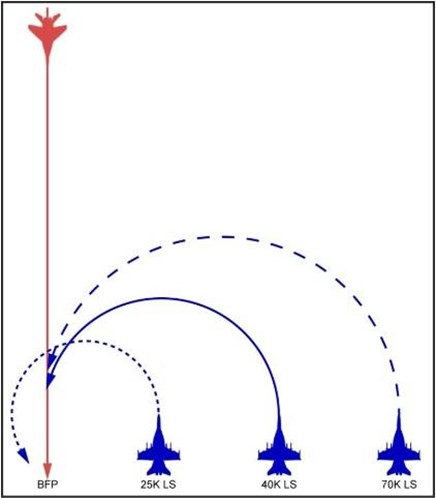
\includegraphics[width=\textwidth,align=t]{bvr/stern-conversion}
}

\subsubsection*{Process}

\begin{itemize}
  \item "Point and assess". Turn nose on to bogey and check closure, aspect and
    bandit heading

  \item "Offset and position". Check 20 or more degrees to one side.

  \item Follow timeline calls

  \item Assess ID and classification

\end{itemize}

\subsubsection*{Examples}

\textbf{FL RIO (Pri):} "Spectre 1 put them 20 left"\\
\textbf{FL RIO (Pri):} "Spectre 1, set throttles for 450kts"
